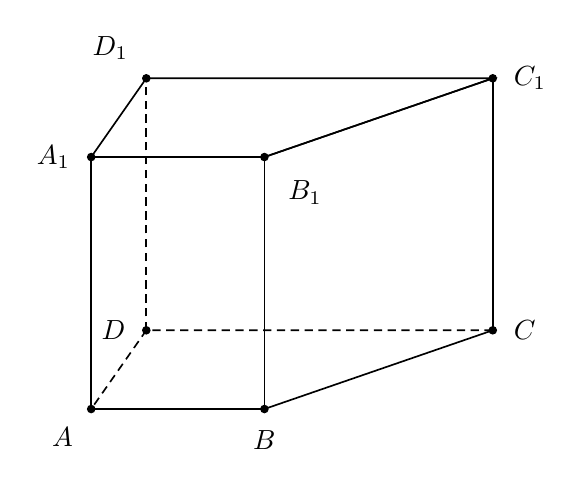
\begin{tikzpicture}[x=1cm,y=1cm,line width=.6pt]
\tikzset{pt/.style={circle,fill=black,inner sep=1.1pt}}
\coordinate (A) at (0,0);
\coordinate (B) at (2.2,0);
\coordinate (D) at (0.7,1.0);
\coordinate (C) at (5.1,1.0);
\coordinate (A1) at (0,3.2);
\coordinate (B1) at (2.2,3.2);
\coordinate (D1) at (0.7,4.2);
\coordinate (C1) at (5.1,4.2);
\draw[black] (A)--(B)--(C);
\draw[black,densely dashed] (C)--(D)--(A);
\draw[black] (A1)--(B1)--(C1)--(D1)--cycle;
\draw[black] (A)--(A1);
\draw[black] (B)--(B1);
\draw[black] (C)--(C1);
\draw[black,densely dashed] (D)--(D1);
\draw[black] (B1)--(C1);
\foreach \p in {A,B,C,D,A1,B1,C1,D1}{\node[pt] at (\p) {};}
\node[below left=3pt] at (A) {$A$};
\node[below=4pt] at (B) {$B$};
\node[right=4pt] at (C) {$C$};
\node[left=4pt] at (D) {$D$};
\node[left=4pt] at (A1) {$A_{1}$};
\node[below right=5pt] at (B1) {$B_{1}$};
\node[right=4pt] at (C1) {$C_{1}$};
\node[above left=3pt] at (D1) {$D_{1}$};
\end{tikzpicture}

